\documentclass[a4paper,12pt, oneside]{book}

% \usepackage{fullpage}
\usepackage[italian]{babel}
\usepackage[utf8]{inputenc}
\usepackage{amssymb}
\usepackage{amsthm}
\usepackage{graphics}
\usepackage{amsfonts}
\usepackage{listings}
\usepackage{amsmath}
\usepackage{amstext}
\usepackage{engrec}
\usepackage{rotating}
\usepackage{verbatim}
\usepackage[safe,extra]{tipa}
\usepackage{showkeys}
\usepackage{multirow}
\usepackage{hyperref}
\usepackage{microtype}
\usepackage{fontspec}
\usepackage{enumerate}
\usepackage{braket}
\usepackage{marginnote}
\usepackage{pgfplots}
\usepackage{cancel}
\usepackage{polynom}
\usepackage{booktabs}
\usepackage{enumitem}
\usepackage{framed}
\usepackage{pdfpages}
\usepackage{pgfplots}
\usepackage{algorithm}
% \usepackage{algpseudocode}
\usepackage[cache=false]{minted}
\usepackage{mathtools}
\usepackage[noend]{algpseudocode}
\usepackage{tikz}\usetikzlibrary{er}\tikzset{multi  attribute /.style={attribute
    ,double  distance =1.5pt}}\tikzset{derived  attribute /.style={attribute
    ,dashed}}\tikzset{total /.style={double  distance =1.5pt}}\tikzset{every
  entity /.style={draw=orange , fill=orange!20}}\tikzset{every  attribute
  /.style={draw=MediumPurple1, fill=MediumPurple1!20}}\tikzset{every
  relationship /.style={draw=Chartreuse2,
    fill=Chartreuse2!20}}\newcommand{\key}[1]{\underline{#1}} 


\usepackage{fancyhdr}
\pagestyle{fancy}
\fancyhead[LE,RO]{\slshape \rightmark}
\fancyhead[LO,RE]{\slshape \leftmark}
\fancyfoot[C]{\thepage}


\title{Metodi Formali}
\author{UniShare\\\\Davide Cozzi\\\href{https://t.me/dlcgold}{@dlcgold}}
\date{}

\pgfplotsset{compat=1.13}
\begin{document}
\maketitle

\definecolor{shadecolor}{gray}{0.80}
\setlist{leftmargin = 2cm}
\newtheorem{teorema}{Teorema}
\newtheorem{definizione}{Definizione}
\newtheorem{esempio}{Esempio}
\newtheorem{corollario}{Corollario}
\newtheorem{lemma}{Lemma}
\newtheorem{osservazione}{Osservazione}
\newtheorem{nota}{Nota}
\newtheorem{esercizio}{Esercizio}
\algdef{SE}[DOWHILE]{Do}{doWhile}{\algorithmicdo}[1]{\algorithmicwhile\ #1}
\tableofcontents
\renewcommand{\chaptermark}[1]{%
  \markboth{\chaptername
    \ \thechapter.\ #1}{}}
\renewcommand{\sectionmark}[1]{\markright{\thesection.\ #1}}
\newcommand{\floor}[1]{\lfloor #1 \rfloor}

\chapter{Introduzione}
\textbf{Questi appunti sono presi a lezione. Per quanto sia stata fatta
  una revisione è altamente probabile (praticamente certo) che possano
  contenere errori, sia di stampa che di vero e proprio contenuto. Per
  eventuali proposte di correzione effettuare una pull request. Link: }
\url{https://github.com/dlcgold/Appunti}.\\
\textbf{Grazie mille e buono studio!}
\section{Contenuti del Corso}
\textit{Il corso tratta di metodi e tecniche formali per specificare, disegnare e
  analizzare sistemi complessi, in particolare sistemi concorrenti e distribuiti
  costituiti da componenti che operano in modo indipendente e che interagiscono
  tra loro.} \\ \\
Si usa un linguaggio logico che spiega il comportamento di tali sistemi e fa
riferimento alla \textbf{logica temporale} di tali sistemi, in quanto le
proprietà di tali sistemi sono tali per cui evolvono con il cambiamento di stato
del sistema e quindi serve una logica che descriva le proprietà dell'evoluzione
del comportamento.\\
Si parlerà delle \textbf{Reti di Petri}, ovvero uno strumento per modellare tali
sistemi concorrenti e distribuiti. Questo modello ha intrinsechi dei teoremi
matematici atti a studiare il comportamento di tali sistemi.\\
In laboratorio si studieranno algoritmi e strumenti software per la modellazione
e l'analisi di tali sistemi.\\
Si introducono a che sistemi dinamici a tempi discreti, come gli \textbf{automi
  cellulari}.
\chapter{Sviluppo di Modelli e Sistemi}
Si hanno diverse fasi di sviluppo di \textit{sistemi complessi} (nel nostro caso
\textbf{concorrenti} e \textbf{distribuiti}). Si hanno 4 grandi fasi (che
riprendono le generiche fasi dello sviluppo software), che non
seguono una rigida sequenza cronologica tra di loro:
\begin{enumerate}
  \item specifica del problema e delle proprietà della soluzione
  \item modellazione della soluzione
  \item implementazione
  \item verifica, validazione e collaudo, sia sul modello che
  implementazione (con eventuali modifiche)
\end{enumerate}
\textbf{Queste fasi possono alternarsi a vicenda}.\\
\textit{I metodi formali possono svolgere una parte rilevante in tutte queste 4
  fasi e hanno la prerogativa di sviluppare questi sistemi in maniera corretta e
  persistente.} \\
Ci si focalizza sulla modellazione e sulla specifica delle proprietà. Si studia
inoltre la verifica delle proprietà sul modello costruito. \textit{In questo
  corso si lascia un attimo da parte l'aspetto implementativo, che comunque
  seguirebbe alla verifica e alla validazione del metodo}.\\
% note sull'utilità dei metodi formali su elearning e sul loro uso
Si hanno diversi modelli di sistemi concorrenti e distribuiti, presenti in
letteratura: 
\begin{itemize}
  \item \textbf{Algebre di Processi}, ovvero una miriade di diversi linguaggi,
  studiate inizialmente da Milner, che introdusse il calcolo dei sistemi
  comunicanti, un calcolo algebrico utile alla semantica della
  concorrenza. Inoltre Hoare ha introdotto i \textbf{processi sequenziali
    comunicanti} come un nucleo di linguaggio di programmazione, usato come
  linguaggio macchina per le prime macchine parallele. Queste algebre si basano
  sul paradigma di avere un forte aspetto della \textbf{composizionalità}, in
  quanto un sistema viene visto come costituito da diverse componenti autonome
  (sia hardware, che software, che umane) che interagiscono tra loro
  sincronizzandosi (in modo sincrono, \textit{handshaking}, sfruttando un ``canale di comunicazione''
  che viene modellato come un processo) e scambiandosi messaggi. Questo
  paradigma è anche alla base dello sviluppo di molti linguaggi di
  programmazione specificatamente dedicati alla concorrenza.
  \item \textbf{Automi a Stati Finiti}. Un modello concorrente e distribuito
  viene spesso rappresentato attraverso \textbf{sistemi di transizioni
    etichettati}, che sono una derivazione del modello degli automi a stati
  finiti, già usati in letteratura per modellare reti neurali, progettare
  circuiti asincroni, modellare macchine a stati finiti, riconoscere linguaggi
  regolari (il teorema di Kleene ci ricorda che \textit{ad un automa a stati
    finiti è possibile associare un'espressione regolare}) e per la modellazione
  di protocolli di comunicazione. 
  \item \textbf{Reti di Petri}, introdotte da Petri con la \textbf{teoria
    generale delle reti di Petri} nella sua tesi di dottorato. Questa teoria
  parte da una critica al modello a stati finiti dove il focus è su stati
  globali e trasformazione di stati globali. Petri cercava invece una teoria
  matematica (fondata sui principi della fisica moderna della relatività e della
  quantistica) che fosse una teoria dei sistemi in grado di descrivere sistemi
  complessi in cui mettere al centro il flusso di informazione e che potesse
  permettere di analizzare l'organizzazione dal punto di vista del flusso di
  informazione che passa da una componente all'altra. Non si ha il focus,
  quindi, su ``macchine calcolatrici'' ma come supporto alla comunicazione in
  organizzazioni complesse. Si hanno quindi diversi elementi chiave:
  \begin{itemize}
    \item la comunicazione
    \item la sincronizzazione tra componenti
    \item il flusso di informazione che passa tra le varie componenti
    \item la relazione di concorrenza e l'indipendenza causale tra i vari eventi
    che comportano i cambiamenti di stato. Ci si concentra su stati locali
    e non sulla visione di una sequenza di azioni e di uno stato globale
  \end{itemize}
  La teoria delle reti di Petri è stata poi sviluppata e ha avuto diverse
  applicazioni. Sono stati sviluppati diversi linguaggi, ovvero diverse
  \textbf{classi di reti di Petri} per descrivere un sistema complesso a livelli
  differenti di astrazione. \\
  Sono state anche sviluppate tecniche formali di analisi e di verifica del
  modello (disegnato mediante reti di Petri), basate sulla teoria dei grafi e
  sull'algebra lineare.\\
  Le reti di Petri hanno avuto un notevole utilizzo in diversi ambiti
  applicativi anche estranei all'informatica pura e allo studio della
  concorrenze, come la modellazione di sistemi biologici o la modellazione di
  reazioni chimiche. Mediante una classe di reti particolare, le \textbf{reti
    stocastiche} si può valutare le prestazioni di un determinato modello.
\end{itemize}
\subsubsection{Sistemi di Transizioni Etichettati}
\begin{definizione}
  I sistemi di transizione etichettati sono definiti come gli automi a stati
  finiti ma senza essere visti come riconoscitori di linguaggi infatti un sistema
  è formato da un insieme, solitamente finito, di stati globali $S$. Si ha poi un
  \textit{alfabeto} delle possibili azioni che può eseguire il sistema. Si hanno
  anche delle relazioni di transizioni, ovvero delle transizioni che permettono di
  specificare come, attraverso un'azione, si passa da uno stato ad un altro. Le
  transizioni si rappresentano con archi etichettati tra i nodi, che rappresentano
  gli stati. Le etichette degli archi rappresentano le azioni necessarie alla
  trasformazione. L'insieme delle azioni viene chiamato $E$ mentre $T\subseteq
  S\times E\times S$ è l'insieme degli archi etichettati. Può essere,
  opzionalmente, individuato uno stato iniziale $s_0$. Un sistema non è obbligato
  a ``terminare'', quindi non si ha obbligatoriamente uno stato finale.\\
  Riassumendo quindi un sistema di transizione etichettato è un quadrupla:
  \[A=(S,E,T,s_0)\]
  \begin{figure}[H]
    \centering
    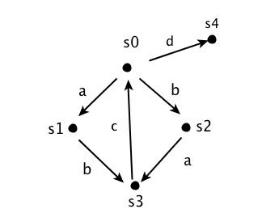
\includegraphics[scale = 0.5]{img/ste.jpg}
    \caption{Esempio di sistema di transizione etichettato}
  \end{figure}
\end{definizione}
La critica di Petri è che in un sistema distribuito non sia individuabile uno
\textbf{stato globale}, che in un sistema distribuito le trasformazioni di stato
siano \textbf{localizzate} e non globali, che non esista un sistema di
riferimento temporale unico (si possono avere più assi temporali in un sistema
distribuito). Quindi la simulazione sequenziale non deterministica (emantica a
``interleaving'') dei sistemi distribuiti è una forzatura e non rappresenta le
reali caratteristiche del comportamento del sistema, ovvero la località, la
distribuzione degli eventi e la relazione di dipendenza causale e non causale
tra gli eventi.
\section{Sistemi Elementari}
Per introdurre i sistemi elementari delle reti di Petri, ovvero una classe molto
semplice e astratta partiamo da un esempio:
\begin{esempio}
  Vediamo l'esempio del \textit{Produttore e del Consumatore}.\\
  Si ha un sistema con una componente Produttore che produce elementi e li
  deposita in un buffer che ha un'unica posizione (quindi o è pieno o è vuoto) e
  con un consumatore che preleva dal buffer un elemento per poi consumarlo ed
  essere pronto a prelevare un altro elemento. Si ha un comportamento
  ciclico. Usiamo quindi le reti di Petri, col modello dei sistemi elementari,
  per rappresentare questo modello. Bisogna quindi individuare le proprietà
  fondamentali locali del sistema.\\
  Partiamo dal produttore, che può avere 2 stati locali:
  \begin{enumerate}
    \item pronto per produrre
    \item pronto per depositare
  \end{enumerate}
  Usiamo i \textbf{cerchi} per rappresentare condizioni locali che sono
  associabili a delle proposizioni della logica che possono essere vere o
  false. Queste preposizioni sono quindi stati locali. Gli eventi locali vengono
  invece rappresentati con un \textbf{rettangolo}. Un evento ha un arco entrante
  da uno stato che rappresenta le \textit{precondizioni} di quell'evento (che
  devono essere vere per permettere l'occorrenza dell'evento). L'occorrenza
  dell'evento rende false le precondizioni e rende vere le
  \textit{postcondizioni} (che sono stati raggiungibili con un arco uscente da
  un evento). Si ha quindi che il produttore può depositare solo se il buffer
  non è pieno, quindi le postcondizioni di un evento devono essere false
  affinché l'evento possa occorrere (oltre alle precondizioni vere).\\
  Passiamo al consumatore che estrae solo se il buffer è pieno ed è pronto a
  prelevare. Si procede poi con la stessa logica del produttore di cambiamento
  tra vero e falso delle varie condizioni locali.\\
  In questo esempio si hanno quindi condizioni che sono preposizioni booleane e
  rappresentano stati locali.
  \begin{figure}[H]
    \centering
    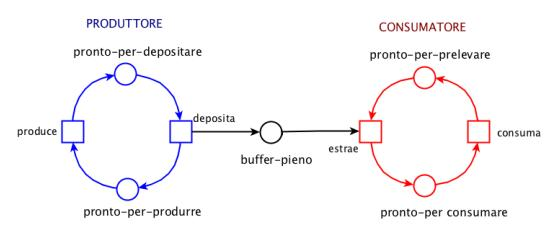
\includegraphics[scale = 0.7]{img/prod.jpg}
    \caption{Produttore e Consumatore}
  \end{figure}
  Lo stato globale del sistema è dato da una
  collezione di stati locali. Per segnare tali condizioni mettiamo un punto
  pieno dentro il cerchio e queste condizioni ``abilitano'' i vari eventi:
  \begin{figure}[h]
    \centering
    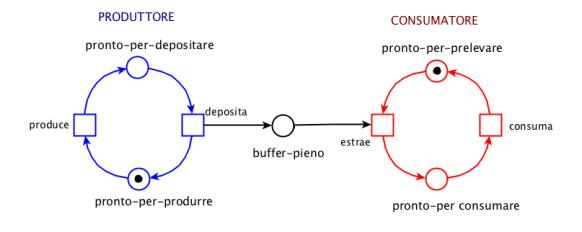
\includegraphics[scale = 0.7]{img/prod1.jpg}
    \caption{Uno stato globale Produttore e Consumatore dove l’evento\textit{
        produce} è l’unico abilitato} 
  \end{figure}
  Si può arrivare ad una \textit{configurazione} dove, per esempio, sia l'evento
  \textit{produce}, del produttore, che l'evento \textit{preleva}, del
  consumatore, sono abilitati. Si ha quindi che i due eventi possono occorrere
  in modo \textbf{concorrente} infatti i due eventi sono \textbf{indipendenti}
  in quanto condizionati da \textbf{precondizioni e postcondizioni completamente
    disgiunte}. Due eventi che occorrono in maniera concorrente lo possono fare in
  qualsiasi ordine, non si ha infatti una sequenza temporale specifica tra i
  due. \\
  In questo sistema quindi siano solo stati locali ed eventi localizzati e non
  stati ed eventi globali. Un evento dipende solo dalle sue precondizioni e
  dalle sue postcondizioni.\\
  \textit{Se rappresentiamo con delle marche le condizioni vere possiamo
    simulare il comportamento del sistema con il \textit{gioco delle marche} che
    mostra come l'evoluzione delle condizioni avviene all'occorrenza degli
    eventi.} \\
  La simula di un tale sistema può comunque avvenire con un sistema di
  transizioni etichettato, ovvero con un automa a stati finiti, che rappresenta
  gli stati globali corrispondenti alle diverse combinazioni di stati locali che
  di volta in volta sono veri. Gli archi vengono etichettati con gli eventi che
  comportano un cambiamento di stato globale:
  \begin{figure}[H]
    \centering
    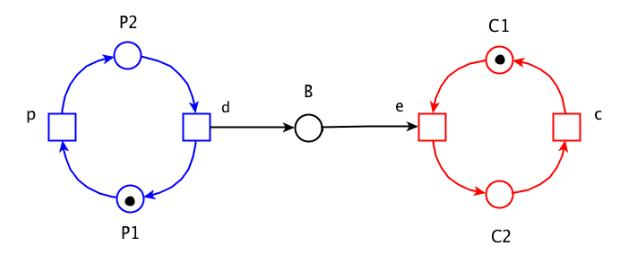
\includegraphics[scale = 0.4]{img/prod3.jpg}
    \caption{Semplificazione della nomenclatura del sistema per praticità}
    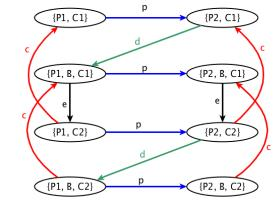
\includegraphics[scale = 0.8]{img/prod2.jpg}
    \caption{Rappresentazione del sistema con un automa a stati finiti che
      rappresenta stati globali}
  \end{figure}
\end{esempio}
Passiamo ora alla formalizzazione di questi aspetti.\\
\begin{definizione}
  Una \textbf{rete elementare} è definita come una tripla:
  \[N=(B,E,F)\]
  dove:
  \begin{itemize}
    \item $B$ è un insieme finito di \textbf{condizioni}, ovvero \textit{stati
      locali}, preposizioni booleane etc$\ldots$. Vengono rappresentate con un
    cerchio 
    \item $E$ è un insieme finito di \textbf{eventi}, ovvero trasformazioni
    locali di stato e \textit{transizioni locali}. Vengono rappresentate con un
    quadrato 
    \item $F$ è una \textbf{relazione di flusso} che connette condizioni ad
    eventi ed eventi a condizioni. Si ha quindi che:
    \[F\subseteq (B\times E)\cup(E\times B)\]
    Le relazioni di flusso sono rappresentate da archi orientati. Inoltre la
    relazione di flusso è tale per cui non esistano \textbf{elementi isolati},
    in quanto non avrebbero senso, in un tale sistema, eventi isolati (che non
    modificherebbero mai una condizione) o condizioni isolate (che non
    verrebbero mai modificate da un evento). Si ha, formalmente, che: 
    \[dom(F)\cup ran(F)=B\cup E\]
    \textbf{chiedere per formula sopra}
  \end{itemize}
  Si ha che:
  \[B\cap E = \emptyset\]
  \[B\cup E \neq \emptyset\]
  Ovvero gli insiemi delle condizioni e degli eventi sono tra loro disgiunti e
  non vuoti.\\
  Sia ora $x$ un elemento qualsiasi della rete, ovvero $x$ può essere o una
  condizione o un evento, formalmente:
  \[x\in B\cup E\]
  si ha che:
  \begin{itemize}
    \item $^\bullet x=\{y\in X:\,(y,x)\inF\}$ rappresenta l'insieme di tutti gli
    elementi $y$ che sono connessi dalla relazione di flusso ad $x$, ovvero si
    ha un arco da $y$ a $x$. Sono quindi i \textbf{pre-elementi} di $x$, ovvero
    le \textit{precondizioni}, se $x$ è un evento, o i \textit{pre-eventi}, se
    $x$ è una condizione
    \item $x^\bullet=\{y\in X:\,(x,y)\inF\}$ rappresenta l'insieme di tutti gli
    elementi $y$ che sono connessi dalla relazione di flusso a partire da $x$,
    ovvero si ha un arco da $x$ a $y$. Sono quindi i \textbf{post-elementi} di
    $x$, ovvero le \textit{postcondizioni}, se $x$ è un evento, o i
    \textit{post-eventi}, se $x$ è una condizione
  \end{itemize}
  Posso estendere questa notazione ad insiemi di elementi. Sia $A$ un insieme
  qualsiasi di elementi, che possono quindi essere sia condizioni che eventi:
  \[A\subseteq B\cup E\]
  Si ha quindi che i pre-elementi dell'insieme $A$ sono rappresentati con:
  \[^\bullet A=\cup_{x\in A} ^\bullet x\]
  ovvero l'unione dei pre-elementi di ogni singolo elemento dell'insieme $A$.\\
  Analogamente si ha che i post-elementi dell'insieme $A$ sono rappresentati
  con: 
  \[A^\bullet=\cup_{x\in A} x^\bullet\]
  ovvero l'unione dei post-elementi di ogni singolo elemento dell'insieme $A$.
  \textit{Nelle reti c'è sempre una relazione di \textbf{dualità} tra due elementi, per
    esempio tra condizioni ed eventi, tra pre-eventi e post-eventi, tra
    pre-condizioni e post-condizioni. Inoltre si ha la caratteristica della
    \textbf{località}, quindi si hanno stati locali e trasformazioni di stato
    locali}
\end{definizione}
La rete $N=(B,E,F)$ descrive la \textit{struttura statica del sistema}, il
comportamento é definito attraverso le nozioni di \textbf{caso (o
  configurazione)} e di \textbf{regola di scatto (o di transizione)}.\\
Una rete può anche essere suddivisa in sotto-reti, seguendo l'esempio sopra si
potrebbe avere una sotto-rete per il produttore, una per il consumatore e anche
una per il buffer.\\
\begin{definizione}
  Un \textbf{caso} (o \textbf{configurazione}) é un insieme di condizioni
  $c\subseteq B$ che rappresentano l’insieme di condizioni vere in una certa
  configurazione del sistema, un insieme di \textbf{stati locali} che
  collettivamente individuano lo \textbf{stato globale} del sistema.\\
  Graficamente le condizioni vere presentano un puntino in mezzo al cerchio
  mentre le condizioni false solo un cerchio vuoto
\end{definizione}
\begin{definizione}
  Sia $N=(B,E,F)$ una rete elementare e sia $c\subseteq B$ una certa
  configurazione (non serve quindi necessariamente conoscere tutto lo stato del
  sistema). La \textbf{regola di scatto} mi permette di stabilire quando
  un evento $e\in E$ è abilitato, ovvero può occorrere, in $c$ sse:
  \[^\bullet e\subseteq c \mbox{ e } e^\bullet \cap c = \emptyset\]
  ovvero sse tutte le precondizioni dell'evento sono vere (e quindi sono
  contenute nella configurazione $c$) e sse tutte le postcondizioni sono false
  (quindi non si hanno intersezioni tra le postcondizioni e la
  configurazione). \\
  L'occorrenza (l'abilitazione) di $e$ in $c$ si denota con la scrittura:
  \[c[e >\]
  Se un evento $e$ è abilitato in $c$, ovvero $c[e >$, si ha che quando $e$
  occorre in $c$ genera un nuovo caso $c'$ e si usa la notazione:
  \[c[e > c'\]
  Si ha quindi che $c'$ è così calcolabile:
  \[c'=(c-^\bullet e)\cup e^\bullet\]
  Ovvero togliendo da $c$ tutte le precondizioni dell'evento $e$ e aggiungendo
  quindi tutte le postcondizioni di $e$
\end{definizione}
Le reti si basano sul \textbf{principio di estensionalità}, ovvero sul fatto che
il cambiamento di stato è locale:
\begin{center}
  \textit{un evento è completamente caratterizzato dai cambiamenti che produce
    negli stati locali, tali cambiamenti sono indipendenti dalla particolare
    configurazione in cui l’evento occorre.}
\end{center}
L'importante è che le precondizioni di un evento siano vere e le postcondizioni
false (siamo comunque interessati solo alla validità delle condizioni che
riguardano l'evento).
\newpage
\begin{esempio}
  Vediamo un esempio esplicativo dove l’evento $e$ è l'unico abilitato, ovvero
  le sue precondizioni sono vere e le sue postcondizioni sono false.\\
  Lo scatto di $e$ rende le precondizioni false e le postcondizioni vere,
  mentre le altre condizioni rimangono inalterate:
  \begin{figure}[H]
    \centering
    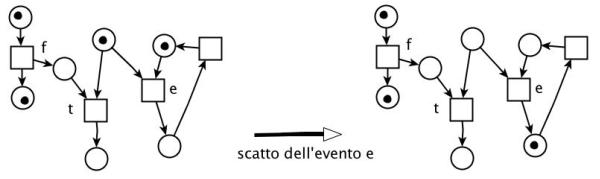
\includegraphics[scale = 0.6]{img/est.jpg}
  \end{figure}
  Si nota quindi che lo scatto dell'evento $e$ riguarda solo le precondizioni e
  le postcondizioni di quel dato evento, come ci ricorda il principio di
  estensionalità 
\end{esempio}
\begin{definizione}
  Sia $N=(B,E,F)$ una rete elementare. Possiamo definire due tipologie di rete:
  \begin{enumerate}
    \item $N$ è definita \textbf{semplice} sse:
    \[\forall x,y \in B\cup E,\,\, (^\bullet x = ^\bullet y)\wedge (x^\bullet =
      y^\bullet)\Rightarrow x = y\]
    Ovvero per ogni coppia di elementi (che siano quindi eventi o condizioni) se
    i loro pre-elementi e i loro post-elementi coincidono allora non ha senso
    distinguere $x$ e $y$.
    \begin{figure}[H]
      \centering
      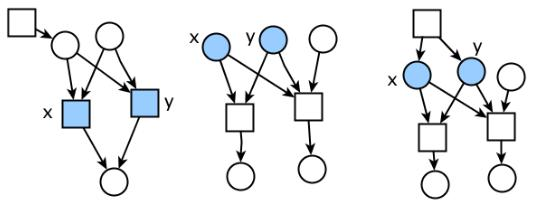
\includegraphics[scale = 0.5]{img/sem.jpg}
      \caption{Esempi di reti \textbf{non} semplici}
    \end{figure}
    \newpage
    \item $N$ è definita \textbf{pura} sse:
    \[\forall e \in E:\,\,^\bullet e \cap e^\bullet = \emptyset\]
    Ovvero se per ogni evento non esiste una precondizione che sia anche
    postcondizioni. Si ha quindi un \textbf{cappio} (detto anche \textbf{side
      condition}) tra un evento e una condizione. Avere questa situazione
    comporta che l'evento non può scattare in quanto la condizione che per lui è
    sia una precondizione che una postcondizioni non può essere
    contemporaneamente vera e falsa, l'evento non potrà mai scattare e quindi
    non potrà mai essere osservato. Non avrebbe quindi senso modellarlo
    \begin{figure}[H]
      \centering
      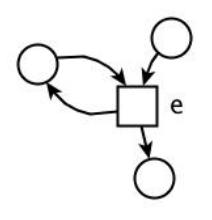
\includegraphics[scale = 0.5]{img/pura.jpg}
      \caption{Esempio di rete \textbf{non} pura}
    \end{figure}
  \end{enumerate}
\end{definizione}
\begin{definizione}
  Data una rete elementare $N=(B,E,F)$ e sia $U \subseteq E$ un sottoinsieme di
  eventi e siano $c,c_1,c_2\in B$ tre configurazioni. Si ha che:
  \begin{itemize}
    \item $U$ è un \textbf{insieme di eventi indipendenti} sse:
    \[\forall e_1,e_2\in U:\,\,e_1\neq e_2\Rightarrow (^\bullet e_1\cup
      e_1^\bullet)\cap  (^\bullet e_2\cup e_2^\bullet) = \emptyset\]
    ovvero per ogni coppia distinta di eventi nell'insieme $U$ si ha che le
    precondizioni e le postcondizioni dei due eventi sono completamente
    disgiunte.
    \item $U$ è un \textbf{passo abilitato}, ovvero un insieme di \textit{eventi
      concorrenti} in una certa configurazione $c$, che si indica con:
    \[c[U>\]
    sse:
    \[U \mbox{ è un insieme di eventi indipendenti } \wedge\,\, \forall e\in
      U:\,\, c[e>\]
    $U$ quindi deve essere un insieme di eventi indipendenti e ogni evento in
    $U$ è abilitato in $c$, quindi le sue precondizioni sono vere e le sue
    postcondizioni sono false. Si ha quindi che $U$ è un insieme di eventi
    abitati in maniera concorrente in $c$
    \item $U$ è un \textbf{passo} dalla configurazione $c_1$ alla configurazione
    $c_2$, che si indica con:
    \[c_1[U > c_2\]
    sse:
    \[(c_1[U) \wedge \Big(c_2=(c_1-^\bullet U)\cup U^\bullet\Big)\]
    ovvero sse $U$ è un passo abilitato in $c_1$ e lo scatto degli eventi in $U$
    porta alla configurazione $c_2$ che si ottiene togliendo da $c_1$ l'insieme
    delle precondizioni degli eventi in $U$ e aggiungendo quindi l'insieme delle
    postcondizioni degli eventi in $U$
  \end{itemize}
\end{definizione}
\begin{esempio}
  Riprendiamo l'esempio del produttore e del consumatore.\\
  Sia dato il sistema $\Sigma$ che modella produttore e consumatore
  \begin{figure}[H]
    \centering
    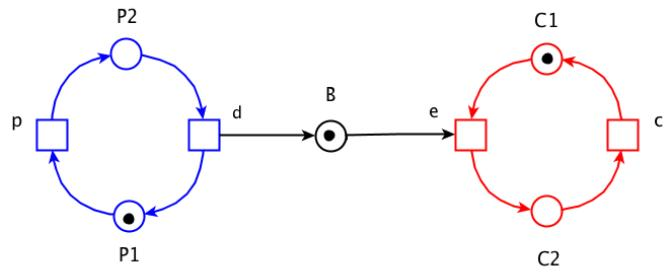
\includegraphics[scale = 0.6]{img/prod5.jpg}
  \end{figure}
  Si hanno:
  \begin{itemize}
    \item $\{p,e\},\{p,c\},\{d,c\}$ esempi di insiemi di eventi indipendenti
    \item $\{p,e\}$ che è un passo abilitato in $\{P_1,B,C_1\}$
    \item $\{P_1,B,C_1\}[\{p,w\}>\{P_2,C_2\}$ ovvero lo scatto del passo
    $\{p,e\}$ ci porta in $\{P_2,C_2\}$
  \end{itemize}
\end{esempio}
Diamo ora una definizione formale di \textbf{sistema elementare}.
\begin{definizione}
  Un \textbf{sistema elementare} $\Sigma=(B,E,F;c_{in})$ è definito come una
  rete $N=(B,E,F)$ e a cui è associato un caso iniziale, una configurazione
  iniziale, ovvero un sottoinsieme di condizioni che rappresentano lo stato
  iniziale da cui inizia la computazione e l'evoluzione del sistema. Formalmente
  il caso iniziale si indica con $C_{in}\in B$ 
\end{definizione}
\begin{definizione}
  Dato un sistema elementare $\Sigma=(B,E,F;c_{in})$ si indica con $C_\Sigma$
  l'insieme dei \textbf{casi raggiungibili} da tale sistema a partire dal caso
  iniziale $c_{in}$.\\
  Formalmente l'insieme dei casi raggiungibili è il di piccolo sottoinsieme
  dell'insieme delle parti di $B$, ovvero $2^B$, tale che:
  \begin{itemize}
    \item $c_{in}\in C_\Sigma$, ovvero sicuramente il caso iniziale appartiene
    all'insieme dei casi raggiungibili
    \item se $c\in C_\Sigma,\,U\subseteq E$ e $c'\subseteq B$ sono tali che
    $c[U>c'$ allora $c'\in C_\Sigma$, ovvero se ho un generico caso $c$ che
    appartiene ai casi raggiungibili, se ho un insieme di eventi $U$ tale che
    questo insieme di eventi (che abbiamo visto essere indipendenti, per la
    definizione di passo abilitato) è abilitato
    in $c$ in un unico passo e la sua occorrenza mi porta in $c'$, allora anche
    $c'$ appartiene a $C_\Sigma$. 
  \end{itemize}
  Questa è una definizione data per \textbf{induzione strutturale}, nel primo
  punto si ha la base, nel secondo l'ipotesi e la conseguenza
\end{definizione}
\begin{definizione}
  Dato un sistema elementare $\Sigma=(B,E,F;c_{in})$ si indica con $U_\Sigma$
  l'\textbf{insieme dei passi} di $\Sigma$, ovvero di tutti i possibili insiemi
  di eventi indipendenti che possono occorrere in qualche caso. Formalmente:
  \[U_\Sigma =\{U\subseteq E\,|\,\exists\, c,c'\in C_\Sigma :\, c[U>c'\}\]
  Ovvero l'insieme dei sottoinsiemi di eventi tali per cui esistano due casi
  raggiungibili in $C_\Sigma$ e $U$ è abilitato in $c$ e il suo scatto mi porta
  in $c'$.
\end{definizione}
Definiamo ora il comportamento dei sistemi elementari.
\begin{definizione}
  Sia $\Sigma=(B,E,F;c_{in})$ un sistema elementare e siano $c_i\in C_\Sigma$ ed
  $e_i\in E$.\\
  Definiamo;
  \begin{itemize}
    \item un \textbf{comportamento sequenziale} come una sequenza di eventi che
    possono occorrere dal caso iniziale. Facendo scattare in maniera sequenziale
    gli eventi uno alla volta in $c_n$:
    \[c_{in} [e_1 > c_1 [e_2 > \ldots[e_n > c_n\]
    Scrittura che può essere alleggerita in:
    \[c_{in} [e_1 e_2 \ldots e_n > c_n\]
    Possiamo dire di avere a che fare con una \textbf{simulazione sequenziale
      non deterministica, detta anche \textit{semantica a interleaving}},
    infatti ho più eventi abilitati da prendere uno alla volta
    \item un \textbf{comportamento non sequenziale}, in quanto possiamo anche
    considerare insiemi di eventi, ovvero passi. Considero quindi sequenze di
    passi, avendo a che fare con la \textbf{step semantics}. Non ho quindi una
    simulazione sequenziale non deterministica in quanto dal caso iniziale
    faccio scattare un insieme di eventi, in maniera concorrente (e quindi senza
    ordine specificato), per poi far scattare un altro insieme di eventi fino ad
    arrivare a $c_n$: 
    \[c_{in} [U_1 > c_1 [U_2 > \ldots [U_n > c_n\]
    Scrittura che può essere alleggerita in:
    \[c_{in} [U_1 U_2 \ldots U_n > c_n\]
    Gli insiemi $U_i$ non sono insiemi massimali abilitati ma sottoinsiemi
    indipendenti e abilitati in $c_{in}$.\\
    Posso avere anche un altro tipo di \textbf{comportamento non sequenziale},
    definito da Petri stesso, in una \textbf{semantica ad ordini parziali} in
    cui si definiscono processi non sequenziali. Il comportamento di tale
    sistema viene registrato in una rete di Petri
  \end{itemize}
  In ogni caso si considerano sia sequenze finite che infinite (con cicli) di
  eventi o passi. 
\end{definizione}
\newpage
\begin{esempio}
  Dato il sistema elementare $\Sigma$:
  \begin{figure}[H]
    \centering
    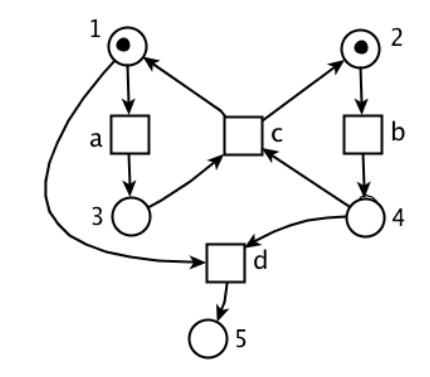
\includegraphics[scale = 0.4]{img/seq.jpg}
  \end{figure}
  si ha, per esempio, la seguente sequenza di occorrenza di eventi:
  \[\{1, 2\}[a > \{3, 2\}[b > \{3, 4\}[c > \{1, 2\}[b > \{1, 4\}[d > \{5\}\]
  arrivati in ``5'' abbiamo un caso finale, ovvero una situazione di
  \textbf{deadlock}, in quanto il sistema non può evolvere ulteriormente.\\
  Vediamo anche la seguente possibile sequenza di passi. In ``1'' e ``2'' sia
  ``a'' che ``b'' sono indipendenti e sono entrambi abilitati (scattano in
  maniera concorrente in un unico passo$\ldots$ ovviamente posso avere passi con lo
  scatto di un solo evento):
  \[\{1, 2\}[\{a, b\} > \{3, 4\}[\{c\} > \{1, 2\}[\{b\} > \{1, 4\}\]
  Come ricordato posso finire in una sequenza infinita.
\end{esempio}
Vediamo ora come modellare e registrare il comportamento del sistema. Un modo è
usando il \textbf{grafo dei casi raggiungibili}.
\begin{definizione}
  Il \textbf{grafo dei casi raggiungibili} di un sistema elementare
  $\Sigma=(B,E,F;c_{in})$ è il sistema di transizioni etichettato:
  \[CG_\Sigma=(C_\Sigma, U_\Sigma, A, c_{in})\]
  dove:
  \begin{itemize}
    \item $C_\Sigma$ è l'insieme dei nodi del grafo, ovvero gli stati globali
    sono i casi raggiungibili dal sistema $\Sigma$    
    \item $U\Sigma$, è l'alfabeto, ovvero i passi del sistema rappresentano
    l'alfabeto 
    \item $A$ è l'insieme di archi etichettati, formalmente definito come:
    \[A=\{(c,U',c')|\,c,c'\in C_\Sigma, U\in U_\Sigma, c[U>c']\}\]
    ovvero sono archi che connettono uno caso $c$ con un caso $c'$ e sono
    etichettati con un passo $U$ sse $U$ è abilitato in $c$ e porta in
    $c'$. Ovviamente $c$ e $c'$ sono devono essere raggiungibili e $U$ deve
    appartenere all'insieme dei passi di $\Sigma$
  \end{itemize} 
\end{definizione}
\begin{figure}[H]
  \centering
  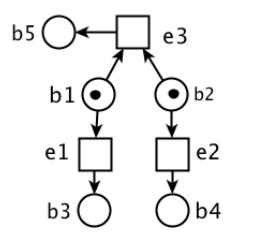
\includegraphics[scale = 0.5]{img/seq1.jpg}
  \caption{il sistema $\Sigma$}
  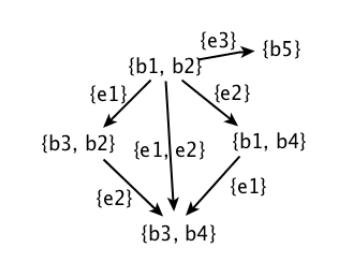
\includegraphics[scale = 0.5]{img/seq2.jpg}
  \caption{Grafo dei casi del sistema $\Sigma$}
\end{figure}
\newpage
\subsection{Diamond Property}
Dato un sistema elementare $\Sigma = (B,E,F;c_{in})$ e il suo grafo dei casi
$CG_\Sigma=(C_\Sigma, U_\Sigma, A, c_{in})$ si ha 
che il grafo soddisfa una particolare proprietà, detta \textbf{diamond
  property}, tipica solo dei sistemi elementari.
\begin{definizione}
  La \textbf{diamond property} stabilisce una proprietà della struttura del
  grafo della rete elementare, ovvero, dati $U_1,U_2\in U_\Sigma$ tali che:
  \begin{itemize}
    \item $U_1\cap U_2=\emptyset$
    \item $U_1\neq\emptyset$
    \item $U_2\neq\emptyset$
  \end{itemize}
  e dati $c_i\in C_\Sigma$ allora vale, per esempio:
  \begin{figure}[H]
    \centering
    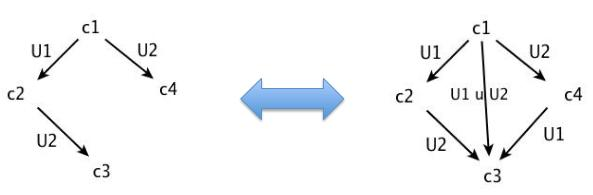
\includegraphics[scale = 0.6]{img/diam.jpg}
  \end{figure}
  ovvero se posso rilevare come sottografo una struttura come quella a sinistra
  nell'immagine allora sicuramente tale sottografo contiene anche l'arco gli
  archi per ottenere l'immagine di destra. Il discorso vale anche all'opposto.
\end{definizione}
Si possono fare delle prove:
\begin{enumerate}
  \item \textbf{prima prova:}\\
  Dimostriamo che possiamo passare all'immagine di destra da quella di sinistra
  aggiungendo i due archi mancanti.\\
  Per semplicità diciamo che $U_i$ è un singolo evento $e_i$, con $i=1,2$. Siano
  inoltre $c_1,c_2\in C_\Sigma$, ovvero sono casi raggiungibili, ed $e_1,e_2\in
  E$ tali che $c_1 [e_1 > c_2 [e_2 > \mbox{ e } c_1 [e_2 >$, i due eventi quindi
  sono abilitati in sequenza e da $c_1$ è anche abilitato $c_2$ . Si vuole
  dimostrare che: 
  \[(^\bullet e_1\cup e_1^\bullet)\cap(^\bullet e_2\cup e_2^\bullet)=\emptyset\]
  ovvero che i due eventi sono indipendenti, che sono entrambi abilitati e che
  sono eseguibili in qualsiasi ordine.
  \newpage
  Da $c_1 [e_1 > \mbox{ e }c_1 [e_2 >$ segue che:
  \begin{itemize}
    \item $^\bullet e_1\cap e_2^\bullet=\emptyset$
    \item $^\bullet e_2\cap e_1^\bullet=\emptyset$
  \end{itemize}
  infatti se $e_1$ e $e_2$ sono entrambi abilitati in $c_1$, le loro
  pre-condizioni sono vere e le post-condizioni false, e quindi non è possibile
  che una condizione sia contemporaneamente precondizione di $e_1$ (vera) e
  anche postcondizione di $e_2$ (falsa), e viceversa. Quindi le precondizioni
  di un evento sono disgiunte dalle postcondizioni dell'altro.\\
  Inoltre dal fatto che ho $c_1 [e_1 > c_2 [e_2$, ovvero che da $c_1$ è
  abilitato $e_1$ e che dopo lo scatto di $e_1$ è ancora abilitato $e_2$
  possiamo dire che:
  \begin{itemize}
    \item $e_1^\bullet\cap e_2^\bullet=\emptyset$
    \item $^\bullet e_1\cap\, ^\bullet e_2=\emptyset$
  \end{itemize}
  in $c_2$, infatti, le pre-condizioni di $e_1$ sono false mentre le
  precondizioni di $e_2$ sono vere e quindi $e_1$ e $e_2$ non possono avere
  precondizioni in comune; inoltre sempre in $c_2$ le postcondizioni di $e_1$
  sono vere, mentre quelle di $e_2$ sono false, e quindi $e_1$ e $e_2$ non
  possono avere post-condizioni in comune. Quindi le precondizioni dei due
  eventi sono disgiunte, come del resto anche le postcondizioni, in quanto i due
  eventi sono sequenziali.\\
  Si è quindi dimostrato che i due eventi hanno precondizioni e postcondizioni
  completamente disgiunte e quindi la tesi è verificata
  \item \textbf{seconda prova:}\\
  Analizzando la situazione:
  \begin{figure}[H]
    \centering
    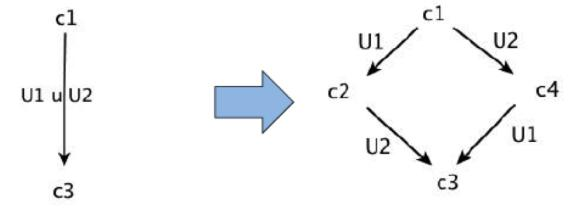
\includegraphics[scale = 0.45]{img/diam2.jpg}
  \end{figure}
  \newpage
  Si supponga che $U_1\cup U_2\in U_\Sigma$ e che si abbiano:
  \begin{itemize}
    \item $U_1\cap U_2=\emptyset$, ovvero sono disgiunti
    \item $U_1\neq\emptyset$
    \item $U_2\neq\emptyset$
  \end{itemize}
  allora se $c_1[(U_1\cup U_2)>c_3$, quindi è abilitato il passo $U_1\cup U_2$
  in $c_1$, sicuramente si ha che sono abilitati anche i singoli passi:
  \begin{itemize}
    \item $c_1[U_1>$
    \item $c_1[U_2>$
  \end{itemize}
  resta da dimostrare che dopo lo scatto di $U_1$ è ancora abilitato $U_2$ in
  $c_2$. Ma se $U_1\cup U_2$ è un passo abilitato significa che posso eseguirli
  in qualsiasi ordine, quindi anche prima $U_1$ e poi $U_2$, e questo comporta
  sicuramente che $U_2$ è abilitato e che porta a $c_3$. Analogamente invertendo
  $U_1$ e $U_2$, formalmente: 
  \begin{itemize}
    \item $c_1[U_1>c_2[U_2>c_3$
    \item $c_1[U_2>c_4[U_1>c_3$
  \end{itemize}
  Si dimostra così che l'immagine di sinistra comporta quella di destra.
\end{enumerate}
Grazie alla diamond property possiamo non considerare il grafo dei casi
raggiungibili ma solo il \textbf{grafo dei casi sequenziale}:
\begin{definizione}
  Un \textbf{grafo dei casi sequenziale} del sistema elementare
  $\Sigma=(B,E,F;c_{in})$ è una quadrupla:
  \[SCG_\Sigma=(C_\Sigma,E,A,c_{in})\]
  dove le etichette sono i singoli eventi (mentre il resto rimane definito come
  nel grafo dei casi raggiungibili). Formalmente si ha quindi che:
  \[A=\{(c,e,c')|,\c,c'\inC_\Sigma,e\in E:\, c[e>c'\}\]
  \begin{figure}[H]
    \centering
    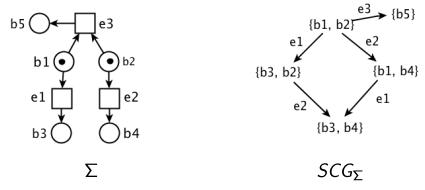
\includegraphics[scale = 0.5]{img/seq3.jpg}
    \caption{Esempio di grafo dei casi sequenziale}
  \end{figure}
  Si registra quindi l'occorrenza di un evento alla volta. Il grafo dei casi
  sequenziale è quindi il sistema di transizione con gli archi etichettati dai
  singoli eventi.
  \begin{figure}[H]
    \centering
    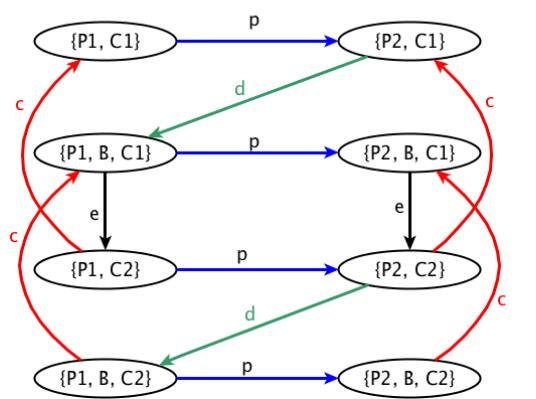
\includegraphics[scale = 0.4]{img/seqq.jpg}
    \caption{Esempio di grafo dei casi sequenziale dell'esempio c0on produttore
      e consumatore}
  \end{figure}
\end{definizione}
Riprendendo l'immagine precedente si ha che per la diamond property possono
aggiungere l'arco ``centrale'' che trasformerebbe nuovamente il grafo dei casi
sequenziale in quello dei casi raggiungibili quindi:
\textit{per la diamond property, nei sistemi elementari il grafo dei casi e il
  grafo dei casi sequenziale sono \textbf{sintatticamente equivalenti}, ovvero
  possono essere ricavati a vicenda.\\
  Questo implica il fatto che due sistemi elementari hanno grafi dei casi
  \textbf{isomorfi} sse hanno grafi dei casi sequenziali isomorfi.}
\subsection{Isomorfismo tra Sistemi di Transizione Etichettati}
Si ricorda che:
\begin{center}
  \textit{Si parla di isomorfismo quando due strutture complesse si possono
    applicare l'una sull'altra, cioè far corrispondere l'una all'altra, in modo
    tale che per ogni parte di una delle strutture ci sia una parte
    corrispondente nell'altra struttura; in questo contesto diciamo che due
    parti sono corrispondenti se hanno un ruolo simile nelle rispettive
    strutture.}
\end{center}
Diamo ora una definizione formale di isomorfismo tra sistemi di transizione
etichettati, che possono quindi essere grafi dei casi o grafi dei casi
sequenziali.
\begin{definizione}
  Siano dati due sistemi di transizione etichettati:\\
  $A_1 = (S_1,E_1,T_1,s_{01})$ e $A_2 = (S_2 , E_2 , T_2 , s_{02})$.\\
  e siano date due \textbf{mappe biunivoche}:
  \begin{enumerate}
    \item $\alpha:S_1\to S_2$, ovvero che passa dagli stati del primo sistema a
    quelli del secondo
    \item $\beta:E_1\to E_2$, ovvero che passa dagli eventi del primo sistema a
    quelli del secondo
  \end{enumerate}
  allora:
  \[\langle \alpha,\beta\rangle:A_1= (S_1 , E_1 , T_1 ,s_{01})\to A_2 = (S_2 ,
    E_2 , T_2 , s_{02})\]
  è un \textbf{isomorfismo} sse:
  \begin{itemize}
    \item $\alpha(s_{01})=s_{02}$, ovvero l'immagine dello stato iniziale del
    primo sistema coincide con lo stato iniziale del secondo
    \item $\forall s,s'\in S_1,\forall e\in E_1:\,(s,e,s')\in T_1
    \Leftrightarrow (\alpha(s),\beta(e),\alpha(s'))\in T_2$ ovvero per ogni
    coppia di stati del primo sistema, tra cui esiste un arco etichettato $e$,
    vale che esiste un arco, etichettato con l'immagine di $e$, nel secondo
    sistema che va dall'immagine del primo stato considerato del primo sistema
    all'immagine del secondo stato considerato del secondo sistema, e viceversa
  \end{itemize}
\end{definizione}
\begin{definizione}
  Si definiscono due \textbf{sistemi equivalenti} sse hanno grafi dei casi
  sequenziali, e quindi di conseguenza anche grafi dei casi, \emph{isomorfi}.\\
  Due sistemi equivalenti accettano ed eseguono le stesse sequenze di eventi
\end{definizione}
\subsection{Il Problema della Sintesi}
Si presenta ora un problema tipico dell'informatica, il \textbf{problema della
  sintesi}, ovvero dato un comportamento, o meglio una sua specifica, decidere
se esiste un'implementazione di tale specifica, ovvero un modello, che abbia
esattamente quel comportamento.\\
In questo caso dato un sistema di transizioni etichettato $A=(S,E,T,s_0)$, con:
\begin{itemize}
  \item $S$ insieme degli stati
  \item $E$ insieme delle etichette, ovvero degli eventi
  \item $T$ insieme delle transizioni
  \item $s_0$ stato iniziale
\end{itemize}
ci si propone di stabilire se esiste un sistema elementare
$\Sigma=(B,E,F;c_{in})$, tale che l'insieme degli eventi del sistema esattamente
l'insieme delle etichette di $A$ e tale che il suo grafo dei casi $SCG_\Sigma$
sia isomorfo ad $A$. Ci si propone anche di costruirlo.\\
Il problema è stato risolto mediante la cosiddetta \textbf{teoria delle regioni}
(che però non verrà trattato nel corso). Si può però dire che $A$ dovrà
soddisfare la diamond property, in quanto altrimenti non sarebbe un sistema di
transizioni che potrebbe corrispondere al comportamento di un sistema
elementare.
\subsection{Contatti}
\begin{definizione}
  Sia $\Sigma = (B,E,F;c_{in})$ un sistema elementare e siano $e\in E$ un evento
  e $c\in C_\Sigma$ un caso raggiungibile dal caso iniziale. Allora si ha che
  $(e,c)$ è un \textbf{contatto} sse:
  \[^\bullet e\subseteq c \wedge e^\bullet \cap c \neq\emptyset\]
  Ovvero, in termini pratici, siamo nel caso in cui un evento $e$ ha le
  precondizioni vere, si ha quindi che $^\bullet e\subseteq c$, e l'evento non
  ha tutte le postcondizioni false, quindi $e^\bullet \cap c \neq\emptyset$,
  allora si dice che l'evento $e$ è in una situazione di contatto e quindi non
  può scattare
  \begin{figure}[H]
    \centering
    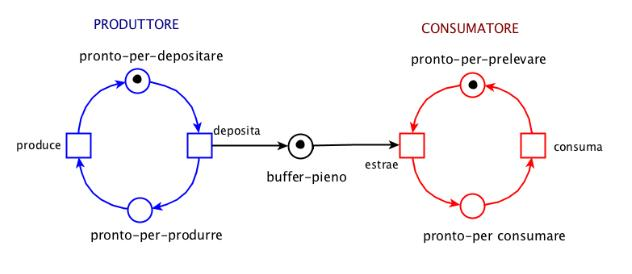
\includegraphics[scale = 0.6]{img/con.jpg}
    \caption{Esempio dove l'evento \emph{deposita} è in una situazione di
      contatto}
  \end{figure}
\end{definizione}
\begin{definizione}
  Sia $\Sigma = (B,E,F;c_{in})$ un sistema elementare. Si dice che il sistema è
  \textbf{senza contatti} sse:
  \[\forall e\in E,\,\forall c\in C_\Sigma\mbox{ si ha che } ^\bullet
    e\subseteq c\Rightarrow e^\bullet\cap c=\emptyset\]
  ovvero per ogni evento e per ogni caso raggiungibile dal caso iniziale succede
  sempre che se le precondizioni sono vere, ovvero $^\bullet e\subseteq c$,
  allora le postcondizioni sono false, ovvero disgiunte dal caso considerato
  ($e^\bullet\cap c=\emptyset$)
\end{definizione}
Ci si chiede se sia possibile trasformare un sistema elementare $\Sigma$, con
contatti, in uno $\Sigma'$, senza contatti, senza però modificarne il
comportamento.\\
La risposta a questo quesito è affermativa e la procedura consiste
nell'aggiungere a $\Sigma$ il complemento di ogni condizione che crea situazione
di contatto, ottenendo così un sistema $\Sigma'$ con grafo dei casi isomorfo a
quello di $\Sigma$.\\ 
Per aggiungere il complemento, data la condizione $x$, si aggiunge la condizione
$not\,\, x$ che sarà vera tutte le volte che $x$ è falsa e viceversa. Per
ottenere questo risultato la nuova condizione avrà come pre-eventi i
post-eventi di $x$ e come post-eventi i pre-eventi di $x$. Ovvero
connetto la nuova condizione agli stessi eventi di quella vecchia ma con archi
orientati in senso opposto. Ovviamente le inizializzazioni delle due condizioni
dovranno essere opposte (una vera e l'altra falsa).
\begin{figure}[H]
  \centering
  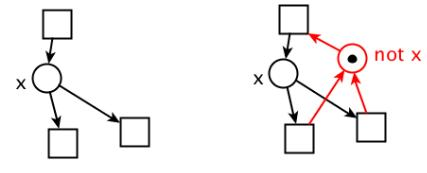
\includegraphics[scale = 0.6]{img/con2.jpg}
  \caption{Esempio con l'ottenimento del complemento di un sistema}
\end{figure}
Se un sistema è senza contatti si ha una regola di contatto semplificata:
\begin{definizione}
   Sia $\Sigma = (B,E,F;c_{in})$ un sistema elementare \textbf{senza
     contatti}. Sapendo che se le precondizioni di un evento sono vere allora
   sicuramente le postcondizioni di quell'evento sono false in quel caso. Dato
   che questo avviene per ogni evento e per ogni caso raggiungibile dal caso
   iniziale per verificare che un evento $e$ sia abilitato in un caso
   raggiungibile $c$ è sufficiente verificare che le precondizioni di $e$ siano
   vere (in quanto automaticamente le postcondizioni saranno false). In
   maniera formale quindi si ha che: 
   \[c[e\mbox{ sse } ^\bullet e\subseteq c,\,\,\mbox{ con } e\in E,c\in
     C_\Sigma\]
   semplificando di molto la \textbf{regola di scatto}
 \end{definizione}
 \begin{figure}[H]
  \centering
  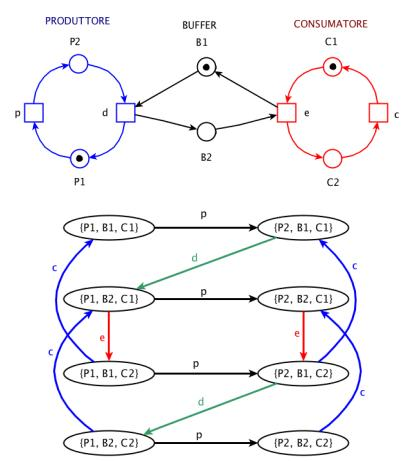
\includegraphics[scale = 0.6]{img/con3.jpg}
  \caption{Esempio con il complemento del sistema produttore-consumatore (dove è
    stato aggiunto solo il complemento di ``buffer-pieno'', ottenendo così sia
    $B1$ che $B2$, in quanto le altre condizioni avevano già il loro
    complemento). In aggiunta si ha anche il grafo dei casi sequenziale
    corrispondente al nuovo sistema senza contatti (grafo che è isomorfo a
    quello ottenibile al sistema con contatti)} 
\end{figure}
\subsection{Situazioni Fondamentali}
\subsubsection{Sequenza}
\begin{definizione}
  Sia $\Sigma = (B,E,F;c_{in})$ un sistema elementare, con contatti o meno
  e siano $c\in C_\Sigma$ un caso raggiungibile dal caso iniziale e $e_1,e_2\in
  E$ due eventi.\\
  Si ha che $e_1$ ed $e_2$ sono \textbf{in sequenza} nel caso
  raggiungibile $c$ sse:
  \[c[e_1>\wedge\, \neg c[e_2\wedge c[e_1e_2>\]
  ovvero in $c$ è abilitato $e_1$ ma non $e_2$ ma, dopo lo scatto di $e_1$,
  $e_2$ diventa abilitato. Quindi in $c$ è possibile attivare prima $e_1$ e poi
  $e_2$ in sequenza.\\
  Si ha quindi una relazione di \textbf{dipendenza causale tra $e_1$ ed $e_2$},
  ovvero qualche postcondizione di $e_1$ è precondizione di $e_2$ (che quindi
  può occorrere solo se precedentemente è occorso $e_1$).
  \begin{figure}[H]
    \centering
    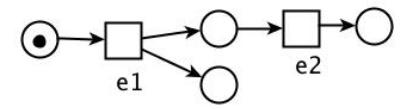
\includegraphics[scale = 0.6]{img/se.jpg}
    \caption{Esempio di sequenza tra $e_1$ ed $e_2$}
  \end{figure}
\end{definizione}
\subsubsection{Concorrenza}
\begin{definizione}
  Sia $\Sigma = (B,E,F;c_{in})$ un sistema elementare, con contatti o meno
  e siano $c\in C_\Sigma$ un caso raggiungibile dal caso iniziale e $e_1,e_2\in
  E$ due eventi. \\
  Si ha che i due eventi sono \textbf{concorrenti} nel caso
  raggiungibile $c$ sse:
  \[c[\{e_1,e_2\}>\]
  ovvero se possono essere abilitati in unico passo o, detto in maniera
  diversa, se sono indipendenti ed entrambi abilitati in $c$
  \begin{figure}[H]
    \centering
    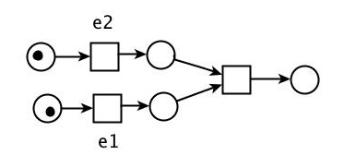
\includegraphics[scale = 0.7]{img/conc.jpg}
    \caption{Esempio di concorrenza tra $e_1$ ed $e_2$}
  \end{figure}
\end{definizione}
\subsubsection{Conflitto}
\begin{definizione}
  Sia $\Sigma = (B,E,F;c_{in})$ un sistema elementare, con contatti o meno
  e siano $c\in C_\Sigma$ un caso raggiungibile dal caso iniziale e $e_1,e_2\in
  E$ due eventi.\\
  Si ha che $e_1$ ed $e_2$ sono in conflitto sse:
  \[c[e_1>\wedge c[e_2 \wedge\,\neg c[\{e_1,e_2\}>\]
  ovvero i due eventi sono entrambi abilitati (quindi le precondizioni sono vere
  mentre le postcondizioni son false) ma l'occorrenza di uno disabilità
  l'altro, quindi non possono essere abilitati in un unico passo, in quanto non
  sono indipendenti. Ci sono due casi:
  \begin{enumerate}
    \item i due eventi hanno una precondizione in comune, e in tal caso si parla
    di \textbf{conflitto forward} (ovvero \textit{in avanti})
    \begin{figure}[H]
      \centering
      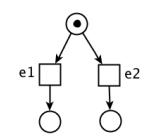
\includegraphics[scale = 0.7]{img/conf1.jpg}
      \caption{Esempio di conflitto forward tra $e_1$ ed $e_2$}
    \end{figure}
    \item i due eventi hanno una postcondizione in comune, e in tal caso si parla
    di \textbf{conflitto backward} (ovvero \textit{all'indietro})
    \begin{figure}[H]
      \centering
      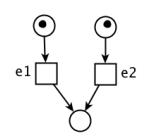
\includegraphics[scale = 0.7]{img/conf2.jpg}
      \caption{Esempio di conflitto backward tra $e_1$ ed $e_2$}
    \end{figure}
  \end{enumerate}
  Si ha quindi una situazione di \textbf{non determinismo}, non essendo
  specificato quale dei due eventi scatterà prima (e lo scatto di uno impedisce
  lo scatto dell'altro).
  \newpage
  Posso ritrovarmi nel caso in cui effettivamente un evento scatta, cambiando lo
  stato del sistema. In tal caso, in un'ottica completamente deterministica, si
  deve assumere che \textbf{l'ambiente} abbia fornito un'informazione
  riguardo il conflitto, ovvero c'è stato qualcosa di esterno che ha permesso ad
  uno dei due eventi di scattare ugualmente. Ho quindi guadagnato
  dell'informazione. 
  \begin{figure}[H]
    \centering
    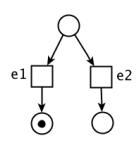
\includegraphics[scale = 0.7]{img/conf3.jpg}
    \caption{Esempio di conflitto con l'intervento dell'ambiente tra $e_1$ ed
      $e_2$ (con conseguente guadagno di informazione)} 
  \end{figure}
  Ci sono però casi in cui in ogni caso non si può avere informazione su quale
  esempio sia scattato. Si può ipotizzare che tale informazione fosse presente
  nello stato precedente del sistema (una sola condizione attiva, per
  esempio). Quindi l'informazione, finita nell'ambiente (ricevuta
  dall'ambiente), si è persa.
   \begin{figure}[H]
    \centering
    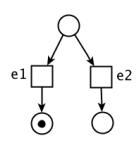
\includegraphics[scale = 0.7]{img/conf3.jpg}
    \caption{Esempio di conflitto tra $e_1$ ed
      $e_2$ con conseguente perdita di informazione (si può ipotizzare, per
      esempio, che nello stato precedente la precondizione di $e_1$ fosse attiva
      mentre quella dio $e_2$ fosse inattiva)} 
  \end{figure}
  Il modello, nell'ottica di Petri, non è quindi un \textbf{modello chiuso} ma è
  in grado di comunicare con l'ambiente (in sintonia con le teorie della
  fisica). 
\end{definizione}
\newpage
\subsubsection{Confusione}
\begin{definizione}
  La situazione di \textbf{confusione} è una \textit{mistura} di situazioni di
  concorrenza e di conflitto. Si hanno 2 tipi di confusione, entrambe
  ammissibili: 
  \begin{enumerate}
    \item detta \textbf{confusione asimmetrica} considera il fatto di avere un
    caso raggiungibile e due eventi abilitati, nella figura $e_1$ ed $e_2$, in
    maniera concorrente in $c$, che nella figura consiste nel caso
    $\{b_1,b_2,b_3\}$. I due eventi sono quindi indipendenti. Nella figura lo
    scatto dei due eventi porterebbe allo stato $c'=\{b_4,b_5\}$. Bisogna
    analizzare però nel dettaglio il sistema. Se prima occorre $e_1$ non si ha
    alcun conflitto mentre se occorre prima $e_2$ (che porterebbe in
    $\{b_1,b_3,b_4\}$) si crea un conflitto tra $e_1$ ed $e_3$, che viene
    risolto a favore di $e_1$ e a sfavore di $e_3$. \textbf{Non è possibile
      stabilire oggettivamente se è stato sciolto un conflitto}. Sono quindi in
    una situazione di confusione in quanto non so se è stata effettuata o meno
    una scelta.
    \begin{figure}[H]
      \centering
      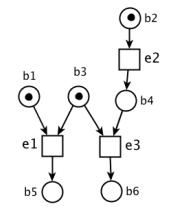
\includegraphics[scale = 0.7]{img/confu.jpg}
      \caption{Esempio di confusione asimmetrica tra $e_1$ ed $e_2$} 
    \end{figure}
    Una soluzione che vedremo sarà la scomposizione in più componenti del
    sistema 
    \item detta \textbf{confusione simmetrica}, nome dovuto al fatto che la rete
    risulta disegnata in modo simmetrico, comportando delle
    problematiche. Prendiamo nell'immagine il caso raggiungibile $c=\{b_1,b_2\}$
    e i due eventi $e_1$ ed $e_3$, abilitati in maniera concorrente. Si ha che
    $c[\{e_1,e_3\}>c'$, con $c'=\{b_3,b_5\}$. Anche in questo caso si hanno dei
    conflitti, infatti sia $e_1$ che $e_3$ sono in conflitto con $e_2$ (in
    quanto se uno dei due viene eseguito $e_2$ non può più occorrere). Anche in
    questo caso non posso stabilire se il conflitto è stato risolto nel momento
    in cui arrivo in $c'$ (ovvero se si è deciso di fare $e_1$ piuttosto che
    $e_2$ o $e_3$ piuttosto che $e_2$).\\
    Anche in questo caso potremo dividere in componenti (una che esegue $e_1$ ed
    $e_2$ e un'altra che esegue $e_1$ ed $e_3$, con $e_2$ che è una
    sincronizzazione tra le due componenti).\\
    Non si può dire chi ha deciso e chi ha la responsabilità di decidere quale
    evento deve occorrere, se alla componente di $b_1$ o a quella di $b_2$.\\
    \begin{figure}[H]
      \centering
      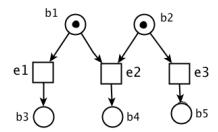
\includegraphics[scale = 0.7]{img/confu2.jpg}
      \caption{Esempio di confusione simmetrica tra $e_1$ ed $e_2$} 
    \end{figure}
  \end{enumerate}
  Petri era convinto, nella sua visione deterministica e senza conflitti, che
  l'avere una situazione di confusione nel modello fosse dovuto al non aver
  esplicitato alcuni aspetti o di aver costruito male il modello, con
  informazioni parziali e non complete sul modello e sull'ambiente.\\
  Un altro studioso, Einar Smith, molto vicino a Petri ha invece dimostrato come la
  confusione sia inevitabile
\end{definizione}
%\newpage
Vediamo un esempio famoso, detto della \textbf{mutua esclusione}, portato da
Smith per spiegare come la confusione sia inevitabile nella realtà.
\begin{esempio}
  Si analizza il seguente sistema:
  \begin{figure}[H]
    \centering
    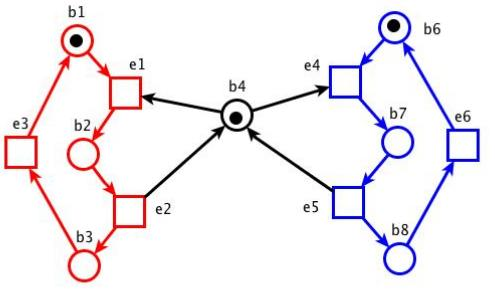
\includegraphics[scale = 0.4]{img/mes.jpg} 
  \end{figure}
  In rosso e in Blu abbiamo specificate le due componenti del sistema, che
  condividono una risorsa, ovvero la condizione $b_4$, che rappresenta che la
  risorsa è libera e a disposizione. L'evento $e_1$ e evento $e_4$ rappresentano
  eventi di acquisizione della risorsa (rispettivamente per la prima e per la
  seconda componente) e quindi le loro precondizioni rappresentano la necessità
  di acquisirla. Tra questi due eventi c'è una \textbf{situazione di
    conflitto}. Le condizioni $b_2$ e $b_7$, ovvero le rispettive postcondizioni
  dei due eventi, rappresentano che la risorsa è in uso per la rispettiva
  componente mentre gli eventi $e_2$ ed $e_5$ rappresentano il rilascio della
  risorsa condivisa, sempre per la rispettiva componente, arrivando
  rispettivamente nella componente $b_3$ e $b_8$. Ovviamente la risorsa
  non può essere contemporaneamente in uso da entrambe le risorse, quindi $b_2$
  e $b_7$ non possono essere contemporaneamente marcate, ovvero vere, e per
  questo si parla di \textit{mutua esclusione} (se una delle due è vera l'altra
  deve essere necessariamente falsa). D'altro canto gli
  eventi $e_3$ ed $e_6$ possono invece occorrere in modo concorrente senza
  conflitti.\\
  Scrivendo formalmente si ha che, nel caso che la risorsa sia stata acquisita
  dalla componente rossa e successivamente rilasciata:
  \[\{b_3,b_4,b_6\}[\{e_3,e_4\}>\{b_1,b_7\}\]
  ma se scatta prima $e_3$ ho il conflitto tra $e_1$ ed $e_4$, se scatta prima
  $e_4$ non ho conflitti con $e_1$. Quindi non ho informazioni sulla risoluzione
  del conflitto.\\
  \textbf{Capire se è confusione simmetrica}
\end{esempio}
\subsection{Sottoreti}
Partiamo subito con una definizione formale:
\begin{definizione}
  Siano $N=(B,E,F)$ e $N_1=(B_1,E_1,F_1)$ due reti elementari.\\
  Si dice che $N_1$ è \textbf{sottorete} di $N$ sse:
  \begin{itemize}
    \item $B_1\subseteq B$, quindi l'insieme delle condizioni della rete $N_1$
    è sottoinsieme di quello della rete $N$
    \item $E_1\subseteq E$, quindi l'insieme degli eventi della rete $N_1$
    è sottoinsieme di quello della rete $N$
    \item $F_1=F\cap[(B_1\times E_1)\cup (E_1\times B_1)]$, ovvero la relazione
    di flusso di $N_1$ è definita come la restrizione della relazione di flusso
    di $N$ rispetto alle condizioni e $B_1$ e agli eventi $E_1$ (tengo quindi solo
    gli archi di $N$ che connettono eventi e condizioni di $N_1$)
  \end{itemize}
\end{definizione}
\begin{definizione}
  Siano $N=(B,E,F)$ e $N_1=(B_1,E_1,F_1)$ due reti elementari.\\
  Si dice che $N_1$ è \textbf{sottorete generata da} $B_1$ di $N$ (ovvero di
  sottorete generata da un insieme di condizioni) sse:
  \begin{itemize}
    \item $B_1\subseteq B$, quindi l'insieme delle condizioni della rete $N_1$
    è sottoinsieme di quello della rete $N$
    \item $E_1=\, ^\bullet B_1\cup B_1^\bullet$, ovvero come eventi si
    hanno tutti quegli eventi che sono collegati in $N$ alle condizioni incluse
    nell'insieme di condizioni $B_1$, prendendo quindi tutti i pre-eventi e i
    post-eventi delle condizioni dell'insieme $B_1$
    \item $F_1=F\cap[(B_1\times E_1)\cup (E_1\times B_1)]$, ovvero la relazione
    di flusso di $N_1$ è definita come la restrizione della relazione di flusso
    di $N$ rispetto alle condizioni $B_1$ e agli eventi $E_1$
  \end{itemize}
  Non ho quindi una sottorete generata da un insieme arbitrario di condizioni ed
  eventi ma questi ultimi sono direttamente presi in relazione all'insieme delle
  condizioni scelto
\end{definizione}
\begin{definizione}
  Siano $N=(B,E,F)$ e $N_1=(B_1,E_1,F_1)$ due reti elementari.\\
  Si dice che $N_1$ è \textbf{sottorete generata da} $E_1$ di $N$ (ovvero di
  sottorete generata da un insieme di condizioni) sse:
  \begin{itemize}
    \item $B_1=\,^\bullet E_1\cup E_1^\bullet$, ovvero come condizioni si
    hanno tutte quelle condizioni che sono collegati in $N$ agli eventi inclusi
    nell'insieme di eventi $E_1$, prendendo quindi tutte e precondizioni e le
    postcondizioni degli eventi dell'insieme $E_1$
    \item $E_1\subseteq E$, quindi l'insieme degli eventi della rete $N_1$
    è sottoinsieme di quello della rete $N$
    \item $F_1=F\cap[(B_1\times E_1)\cup (E_1\times B_1)]$, ovvero la relazione
    di flusso di $N_1$ è definita come la restrizione della relazione di flusso
    di $N$ rispetto alle condizioni $B_1$ e agli eventi $E_1$
  \end{itemize}
  Non ho quindi una sottorete generata da un insieme arbitrario di condizioni ed
  eventi ma le prime sono direttamente prese in relazione all'insieme degli
  eventi scelto
\end{definizione}
\newpage
\begin{esempio}
  Tornando all'esempio della mutua esclusione:
  \begin{figure}[H]
    \centering
    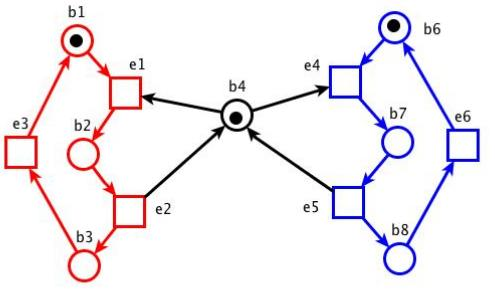
\includegraphics[scale = 0.4]{img/mes.jpg} 
  \end{figure}
  si ha, per esempio:
  \begin{itemize}
    \item in rosso si ha la sottorete $N'=(\{b_1,b_2,b_3\},
    \{e_1,e_2,e_3\},F')$, che è la sottorete generata  dall'insieme di
    condizioni $B'=\{b_1,b_2,b_3\}$ 
    \item in blu si ha la sottorete $N'=(\{b_6,b_7,b_8\},
    \{e_4,e_5,e_6\},F')$, che è la sottorete generata dall'insieme di condizioni
    $B'=\{b_6,b_7,b_8\}$
    \item si ha la sottorete $N'=(\{b_2,b_4,b_7\},\{e_1,e_2,e_4,e_5\},F')$, che
    è la sottorete generata  dall'insieme di condizioni $B'=\{b_2,b_4,b_7\}$
    \item si ha la sottorete $N'=(\{b_1,b_2,b_3,b_4\},\{e_1,e_2,e_3\},F')$, che è la
    sottorete generata da  dall'insieme di eventi $E'=\{e_1,e_2,e_3\}$
  \end{itemize}
\end{esempio}
\subsection{Operazioni di Composizione per Reti di Petri}
Data una rete $N=(B,E,F,c_0)$ questa può essere ottenuta componendo altre reti
di Petri. Si hanno in letteratura 3 modi principali:
\begin{enumerate}
  \item la \textbf{composizione sincrona}
  \item la \textbf{composizione asincrona}
  \item la \textbf{composizione mista, tra sincrona e asincrona}
\end{enumerate}
\newpage
Iniziamo informalmente a vedere degli esempi pratici.
\begin{esempio}
  Supponiamo di avere i modelli di due componenti, $N_1$, con un evento che
  corrisponde ad un'azione di invio, ed $N_2$, con un evento che corrisponde ad
  un'azione di ricezione:
  \begin{figure}[H]
    \centering
    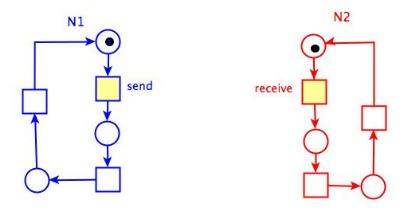
\includegraphics[scale = 0.5]{img/sinc.jpg} 
  \end{figure}
  Supponiamo che invio e ricezione siano eventi corrispondenti all'handshacking,
  ovvero l'invio avviene solo se può avvenire la ricezione.\\
  Vado quindi a sincronizzare questi due eventi, che diventano quindi un'unico
  evento nella rete composta, che è abilitato se le due precondizioni, nelle due
  componenti sono entrambe vere: 
  \begin{figure}[H]
    \centering
    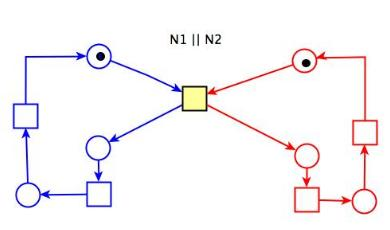
\includegraphics[scale = 0.5]{img/sinc2.jpg} 
  \end{figure}
  La composizione viene indicata con:
  \[N_1||N_2\]
  Lo scatto dell'evento, in maniera sincrona, rende vere le postcondizioni nelle
  due componenti e false le due precondizioni.\\
  Abbiamo appena visto un esempio di \textbf{composizione sincrona}
\end{esempio}
\newpage
\begin{esempio}
  Supponiamo di avere i modelli di due componenti, $N_1$, che invia in un canale
  un messaggio (per esempio in un buffer), e $N_2$, che riceverà il messaggio
  solo quando esso sarà disponibile:
  \begin{figure}[H]
    \centering
    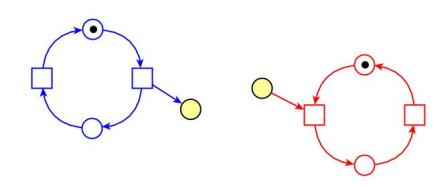
\includegraphics[scale = 0.5]{img/asinc.jpg} 
  \end{figure}
  In questo caso, a differenza dell'esempio precedente, non identifichiamo
  eventi ma condizioni. Identifico quindi il canale (le due condizioni) come uno
  solo, che avrà il pre-evento in una componente e il post-evento nell'altra.\\
  Quindi il pre-evento, nella componente $N_1$, può scattare solo se questa
  nuova condizione condivisa, il canale, è libera, indipendentemente dalla
  componente $N_2$. D'altro canto l'evento in $N_2$ può scattare solo se la
  condizione condivisa è marcata, indipendentemente dallo stato della prima
  componente, liberando il canale di comunicazione.\
  Avvio e ricezione (dopo che il messaggio è stato inviato può essere letto in
  un qualsiasi futuro) non sono sincronizzati e si ha quindi a che fare con
  un esempio di \textbf{composizione asincrona}
\end{esempio}
Sarà interessante studiare come la composizione di due componenti, per esempio,
senza deadlock non comporta, in generale, l'ottenimento di una rete priva di
deadlock.
\newpage
\section{Reti Posti e Transizioni}
Vediamo ora una nuova classe delle \textit{reti di Petri}, detta \textbf{reti
  Posti e Transizioni}, permette di rappresentare un sistema in modo più
compatto, sono una sorta di \textit{ripiegamento} dei sistemi
elementari. Partiamo quindi da un esempio:
\begin{esempio}
  prendiamo in studio sempre il sistema produttore-consumatore:
  Sia nella versione con contatto:
  \begin{figure}[H]
    \centering
    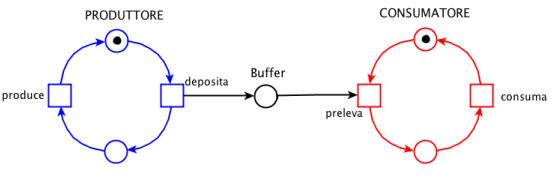
\includegraphics[scale = 0.5]{img/pt.jpg} 
  \end{figure}
  che senza:
  \begin{figure}[H]
    \centering
    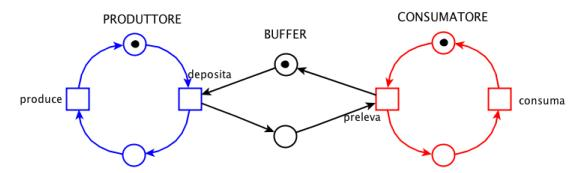
\includegraphics[scale = 0.5]{img/pt2.jpg} 
  \end{figure}
  Suppongo di voler modellare il sistema in modo che il buffer possa avere un
  numero determinato di posizioni, per esempio 2 (il buffer può quindi
  depositare fino a due elementi). Si ottiene quindi:
  \begin{figure}[H]
    \centering
    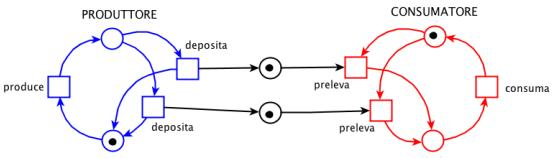
\includegraphics[scale = 0.6]{img/pt3.jpg} 
  \end{figure}
  Dove si hanno due posizioni del buffer (e quindi basta che una sia vuota per
  permettere al produttore di depositare) a disposizione del sistema. Si nota
  come l'aumento dei buffer complica drasticamente la modellazione del sistema.
  Si cerca quindi una soluzione più compatta, compattando gli eventi
  \textit{deposita} e \textit{preleva} e dando nuova notazione al buffer. Si
  ottiene:
  \begin{figure}[H]
    \centering
    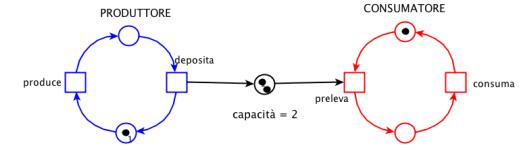
\includegraphics[scale = 0.6]{img/pt4.jpg} 
  \end{figure}
  con il buffer che diventa anche un \textbf{contatore} del numero di elementi
  presenti al suo interno. Un buffer a due posizioni diventa quindi una
  condizione non più booleana, detta \textbf{Posto}, con una \textbf{capacità}
  pari a 2. Il produttore non può produrre oltre la capacità.\\
  Con questa rappresentazione non ho più alcuna difficoltà nel rappresentare più
  posizioni del buffer in quanto basta aumentare la capacità. Ho però perso
  delle informazioni infatti non ho più una relazione di dipendenza tra dove si
  deposita (se nella prima posizione o nella seconda) e dove si preleva.\\
  Aggiungiamo un'altra complicanza: aggiungiamo un secondo consumatore:
  \begin{figure}[H]
    \centering
    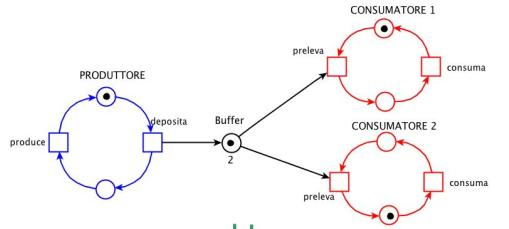
\includegraphics[scale = 0.6]{img/pt5.jpg} 
  \end{figure}
  Possiamo \textit{comprimere} nella stessa maniera, ottenendo, in quanto i due
  consumatori hanno lo stesso modello di comportamento:
  \begin{figure}[H]
    \centering
    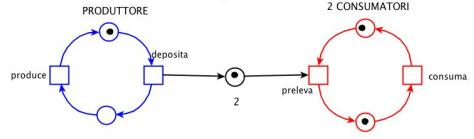
\includegraphics[scale = 0.7]{img/pt6.jpg} 
  \end{figure}
  Anche qui perdo l'informazione riguardo quale dei due consumatori ha
  effettivamente prelevato, riguardo quale dei due è pronto a \textit{prelevare}
  e quale a \textit{consumare}, continuando ad ignorare anche la posizione
  del buffer nei confronti della quale stanno agendo.\\
  Si può arrivare ad avere due componenti identiche che sono concorrenti tra
  loro. 
\end{esempio}
Le condizioni non sono più, in generale, booleane ma sono \textbf{posti}
dotati di \textbf{contatori}, gli elementi all'interno sono detti
\textbf{marche}. Ai posti si assegna anche una \textbf{capacità}. 
\\
Si ha inoltre che lo scatto di una transizione dipende dalla disponibilità
delle risorse, per esempio un produttore può produrre $n$ elementi alla volta
e il consumatore consumarne $m$. Si usano quindi archi pesati (se non indicato
ovviamente ha peso 1, quello del normale check booleano di condizione attiva)
tali che una transizione possa scattare sse i pesi vengono rispettati:
\begin{figure}[H]
  \centering
  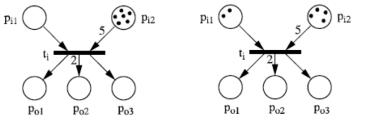
\includegraphics[scale = 0.7]{img/pt7.jpg}
  \caption{Esempi con la transizione $t_i$ non abilitata}
\end{figure}
\begin{figure}[H]
  \centering
  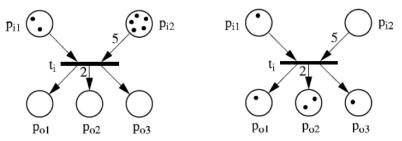
\includegraphics[scale = 0.7]{img/pt8.jpg}
  \caption{Esempio con la transizione $t_i$ abilitata, a sinistra il ``prima''
    e a destra il ``dopo'' lo scatto di $t_i$}
\end{figure}
\newpage
\begin{esempio}
  Petri aveva introdotto l'uso delle reti anche per le reazioni chimiche, per
  esempio:
  \begin{figure}[H]
    \centering
    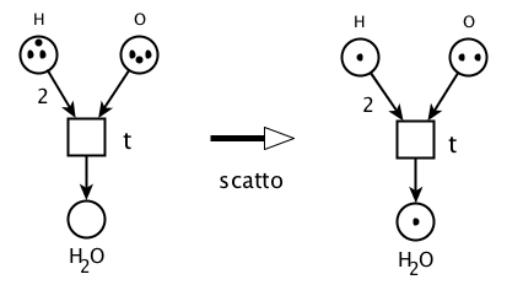
\includegraphics[scale = 0.35]{img/pt9.jpg}
    \caption{Esempio con la modellazione della produzione di $H_2O$}
  \end{figure}
\end{esempio}
\subsection{I Filosofi a Cena}
Questo è un classico problema di sincronizzazione, introdotto da Dijkstra. Si ha
un tavolo rotondo con 5 filosofi ($p_i,\,\i=0,\ldots 4$), ciascuno ha davanti un
piatto di spaghetti e si hanno solo 5 forchette ($f_i,\,\i=0,\ldots 4$):
\begin{figure}[H]
  \centering
  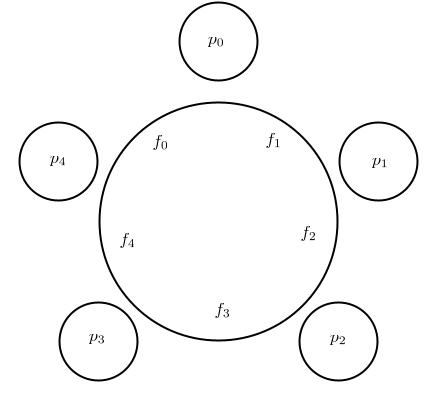
\includegraphics[scale = 0.5]{img/pt10.jpg}
  \caption{Rappresentazione schematica del problema dei 5 filosofi}
\end{figure}
Ogni filosofo ha lo stesso comportamento, un po' pensa e un po' mangia,
prendendo prima la forchetta alla sua destra e poi quella alla sua sinistra
(perché necessitano di due forchette per mangiare). Si ha quindi il
\textit{deadlock} se tutti vogliono mangiare, prendendo tutti in primis una
forchetta, impedendosi tutti a vicenda di mangiare (non potendo prendere due
forchette) o si ha la \textit{starvation} in quanto potrebbero accordarsi per
mangiare in quattro, impedendo a uno di mangiare.\\
Si vuole modellare tale schema. Ogni filosofo può essere modellato come una rete
elementare, che farà da componente al modello finale:
\begin{figure}[H]
  \centering
  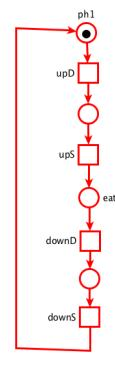
\includegraphics[scale = 0.5]{img/pt11.jpg}
\end{figure}
con gli eventi \textit{upD} e \textit{upS}, dove il filosofo prende la forchetta
destra e sinistra, e rispettivamente \textit{downD} e \textit{downS}, dove le
mette giù. Si ha la condizione che specifica che il filosofo sta pensando e
quella che mi segnala l'azione del mangiare, oltre alle due condizioni
intermedie che separano le azioni tra forchetta sinistra e destra.\\
Si modella anche la componente della forchetta, con gli eventi che segnalano se
è depositata, \textit{down}, o meno, \textit{up}:
\begin{figure}[H]
  \centering
  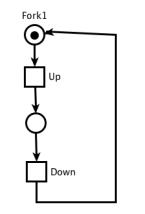
\includegraphics[scale = 0.5]{img/pt12.jpg}
\end{figure}
\newpage
Combino quindi le due componenti per specificare il filosofo che prende la sua
forchetta destra e poi la sinistra, quindi per ogni componente \textit{filosofo}
si hanno due componenti \textit{forchetta}:
\begin{figure}[H]
  \centering
  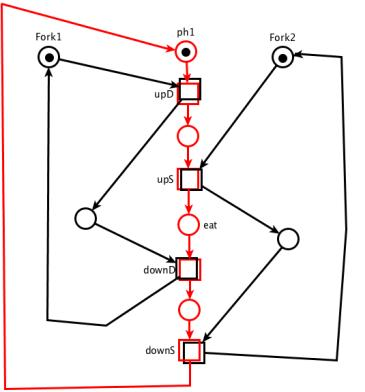
\includegraphics[scale = 0.5]{img/pt13.jpg}
\end{figure}
con la \textit{forchetta 1 (fork 1)} che sarà la forchetta destra e la
\textit{forchetta 2 (fork 2)} che sarà la forchetta sinistra. Si hanno quindi
diverse transizioni di sincronizzazione tra le due componenti (ogni volta che il
filosofo interagisce con la forchetta).\\
Bisogna aggiungere che ogni forchetta può essere presa da due filosofi, ognuna a
destra di un filosofo e a sinistra di un altro:
\begin{figure}[H]
  \centering
  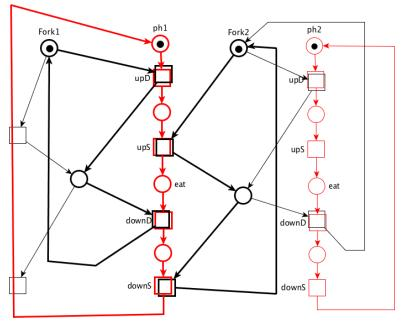
\includegraphics[scale = 0.5]{img/pt14.jpg}
\end{figure}
Ogni forchetta quindi si sincronizza alternativamente tra due filosofi, venendo
presa da uno dei due filosofi. Si è arrivati quindi ad una \textbf{situazione di
  conflitto}, o meglio ad una \textbf{situazione di confusione}.\\
Per ora la soluzione di questo problema viene lasciato da parte per valutare il
modello dello stesso.\\
Si ha quindi una possibile rappresentazione del modello completo:
\begin{figure}[H]
  \centering
  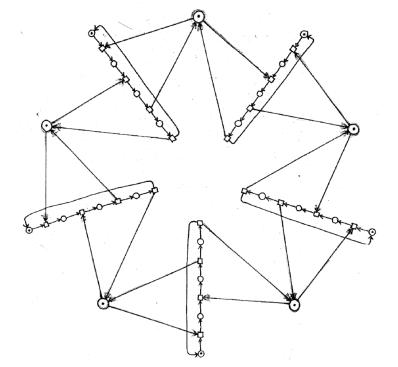
\includegraphics[scale = 0.5]{img/pt15.jpg}
\end{figure}
Ma ogni filosofo, come del resto ogni forchetta, si comporta nella stessa
maniera. Si tenda quindi di \textit{ripiegare} il modello, modellando un
un'unica componente filosofo con 5 marche distribuite nei vari stati locali del
filosofo. Stesso discorso per le forchette. Ottengo quindi il seguente modello:
\begin{figure}[H]
  \centering
  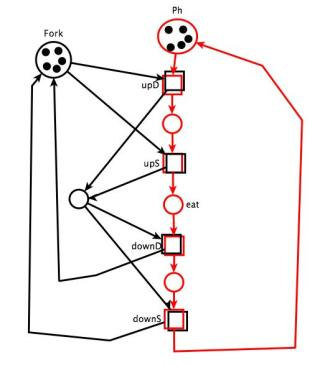
\includegraphics[scale = 0.6]{img/pt16.jpg}
\end{figure}
Con le due componenti, \textit{filosofo} e \textit{forchetta}, entrambe
inizializzate con 5 marche ciascuno. Questo modello però perde informazione
sulla forchetta che un filosofo può prendere, si ha un radicale \textbf{cambio
  di protocollo}. Un filosofo può prendere una qualsiasi forchetta e non più
quella alla sua destra/sinistra. Non posso quindi usare le \textit{reti Posti e
  Transizioni} in quanto perdo troppe informazioni.\\
L'unica soluzione possibile è quindi quella di recuperare le informazioni perse
inserendole nelle marche, alle quali viene aggiunta una struttura dati. Si ha
così modo di distinguere i vari filosofi e le forchette. Per compattare il
sistema devo quindi rendere più complessa l'essenza della marca, viene
arricchita con una struttura dati.\\
Si arriva così ad avere una \textbf{Rete di Alto Livello}, come, per esempio,
una \textit{rete colorata}, a partire da un rete elementare.\\
Distinguo quindi filosofi e forchette nei due insiemi di strutture dati:
\begin{enumerate}
  \item $Phil=\{p_0,\ldots, p_4\}$, insieme dei filosofi
  \item $Fork=\{f_0,\ldots, f_4\}$, insieme delle forchette
\end{enumerate}
Si nota che per gli indici si ha una somma \textit{modulo 5}, ovvero gli indici
rispondono alla regola:
\[(i+1) \mbox{ mod } 5\]
In modo che gli indici siano ordinati avendo inoltre lo 0 che segue il 4, in
modo circolare.\\
Si ottiene quindi, mantenendo il protocollo iniziale:
\begin{figure}[H]
  \centering
  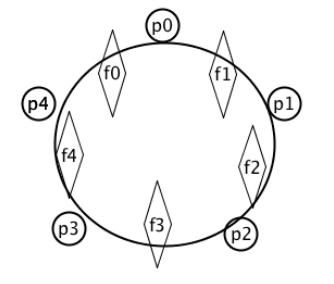
\includegraphics[scale = 0.6]{img/pt17.jpg}
\end{figure}
Si mantiene quindi un modello simile a quello descritto sopra ma al posto di
marche non strutturate si ha nel posto delle 5 forchette le marche dell'insieme
\textit{Fork} e al posto dei 5 filosofi le marche dell'insieme \textit{Phil}:
\begin{figure}[H]
  \centering
  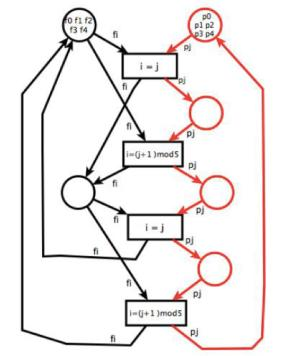
\includegraphics[scale = 0.6]{img/pt18.jpg}
\end{figure}
Le transizioni scattano in determinate condizioni. Per esempio la prima
transizione, relativa al fatto che il filosofo prende la forchetta alla sua
destra, scatta sse con l'istanza filosofo $p_j$ e forchetta $f_i$ si ha che
$i=j$ (ho quindi almeno una forchetta, almeno un filosofo e la forchetta deve
essere quella alla sua destra, che, per come abbiamo modellato il problema, è
quella con lo stesso indice). Sugli archi si hanno quindi annotate determinate
variabili che denotano istanze. Per la forchetta a sinistra si usa il modulo
5. Si procede quindi per i vari filosofi.
\begin{figure}[H]
  \centering
  \includegraphics[scale = 0.5]{img/pt19.jpg}
  \caption{Esempio con il filosofo $p_3$ che ha già preso la forchetta alla sua
    destra, $f_3$, e prende quella a sinistra, $f_4$}
\end{figure}
\textit{Si ha quindi un prezzo per rappresentare in maniera compatta un sistema
  elementare, mediante una rete di alto livello, ovvero l'arricchimento della
  struttura dati}.
\subsection{Formalizzazione delle Reti Posti e Transizioni}
\end{document}

% LocalWords:  postcondizioni LocalWords estensionalità jpg img sse pre sem seq
% LocalWords:  side condition prod interleaving step semantics Petri deadlock
% LocalWords:  Property diamond property sottografo diam postcondizione seqq pt
% LocalWords:  conc conf backward confu mes Smith Einar Sottoreti sottorete upD
% LocalWords:  sinc all'handshacking all'handshacking handshaking asinc primis
% LocalWords:  Dijkstra starvation upS downD downS fork Phil mod
